\documentclass[letterpaper, 12pt]{article}
\usepackage{amsmath}
\usepackage[margin=1in]{geometry}
\usepackage{adjustbox}
\usepackage{graphicx}
\usepackage[final]{pdfpages}
\usepackage{bm}
\usepackage{sectsty}
\usepackage{titlesec}
\usepackage{lipsum}
\usepackage{subcaption}
\usepackage{listings}
\usepackage{pgffor}
\usepackage{rotating}
\usepackage{xcolor}  
\usepackage{amsthm}
\usepackage{csvsimple}
\usepackage{enumitem}
\usepackage{amssymb} 
\usepackage{amsfonts}
\usepackage{tikz}
\usepackage{tikz-3dplot}
% \setlength{\tabcolsep}{0.5cm} 
\newcommand{\thickhat}[1]{\mathbf{\hat{\text{$#1$}}}}
\renewcommand{\lstlistingname}{Program}

\newtheoremstyle{custom}
  {3pt}
  {3pt}
  {\itshape}
  {} 
  {\bfseries}
  {. }  
  { }   
  {\thmname{#1} \thmnumber{#2} \thmnote{ #3}}

\theoremstyle{custom}


\newtheorem{definition}{Definition}
% \newtheorem{theorem}{Theorem}
\newtheorem*{theorem}{Theorem}
\sectionfont{\fontsize{12}{15}\selectfont}
\titleformat{\section}
{\normalfont\normalsize\bfseries}
{(\thesection)}{1em}{}

\title{Inverse Fourier Transform Calculation Example Using Cauchy's Integral Formula}
\date{}
\begin{document}
\maketitle
Although there are several conventions for the Fourier Transform, the following definition is used here.
\begin{equation*}
  \mathcal{F}\left[ f \right] \left( \xi \right) = \frac{1}{\sqrt{2 \pi}} \int_{-\infty}^{\infty} f(x) e^{-i\xi x} \, dx
\end{equation*}

The corresponding inverse Fourier Transform is given by
\begin{equation*}
  \mathcal{F}^{-1}  \left[ \hat{f} \right] \left( x \right) = \frac{1}{\sqrt{2 \pi}} \int_{-\infty}^{\infty} \hat{f}(\xi) e^{i\xi x} \, d\xi
\end{equation*}

As an example, we consider the following function:
\begin{equation*}
  \hat{f}(\xi)  = \frac{1}{\sqrt{2 \pi}} \frac{2a}{a^2+\xi^2}
\end{equation*}

The Inverse Fourier Transform is
\begin{align*}
  \mathcal{F}^{-1}  \left[ \hat{f} \right] \left( x \right) 
  &= \frac{1}{\sqrt{2 \pi}} \int_{-\infty}^{\infty} \hat{f}(\xi) e^{i\xi x} \, d\xi \\
  &= \frac{1}{2 \pi} \int_{-\infty}^{\infty} \frac{2a}{a^2+\xi^2} e^{i\xi x} \, d\xi \\
  &= \frac{1}{2 \pi i} \int_{-\infty}^{\infty} \left[  \frac{1}{\xi-ia} - \frac{1}{\xi+ia}  \right]e^{i\xi x}\, d\xi \\
  &= \frac{1}{2 \pi i} \left[ \int_{-\infty}^{\infty} \frac{e^{i\xi x}}{\xi-ia} \, d\xi -  \int_{-\infty}^{\infty} \frac{e^{i\xi x}}{\xi+ia} \, d\xi \right]
\end{align*}

We can evaluate the integral using Cauchy's integral formula, which is

\begin{equation*}
  f(z_0) = \frac{1}{2 \pi i} \oint_C \frac{f(z)}{z-z_0} \, dz
\end{equation*}
where $f$ is an analytic function within the domain closed by $C$. In addition, $z_0$ is in the domain closed by $C$.
($e^{i\xi x}$ is analytic at any point on the complex plane.)

If $x>0$, we consider the semi-disk shown in Figure \ref{fig1}.

\begin{figure}[htbp]
  \centering
  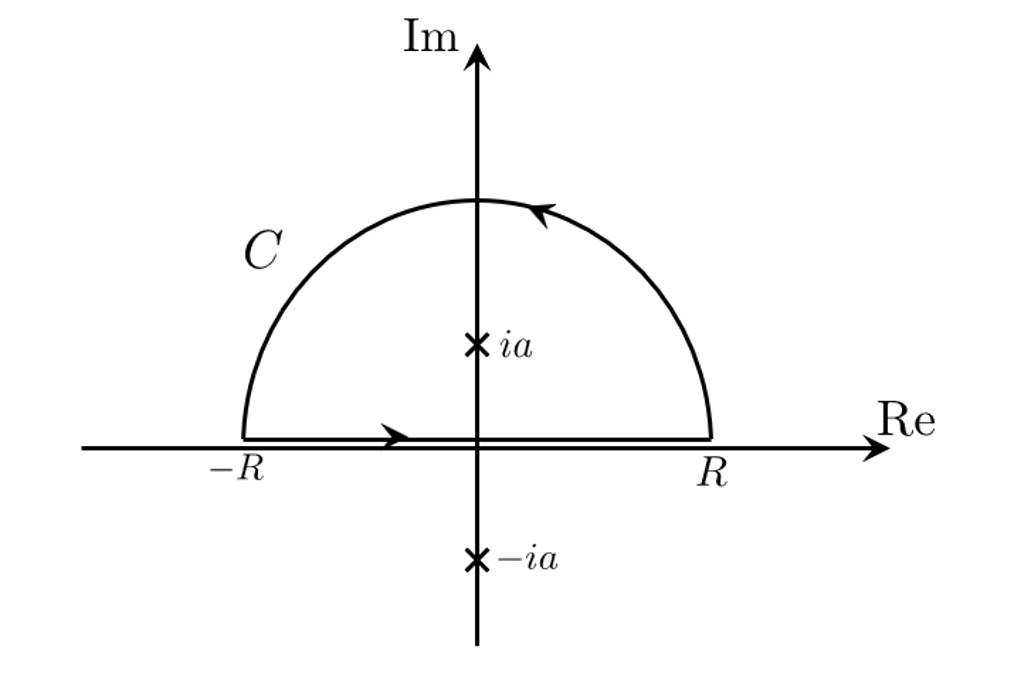
\includegraphics[width=.7\columnwidth]{Contour1.png}
  \caption{Contour $C$ for integration}
  \label{fig1}
\end{figure}

Since there are no singularities for $\displaystyle \frac{e^{izx}}{z+ia}$ inside the contour, we can apply Cauchy's Integral Theorem:
\begin{equation*}
  \frac{1}{2 \pi i} \oint_C \frac{e^{i z x}}{z+ia} \, dz = 0
\end{equation*}

Since $e^{izx}$ does not have singularity inside the contour, we can apply Cauchy's integral formula:
\begin{equation*}
  \frac{1}{2 \pi i} \oint_C \frac{e^{i z x}}{z-ia} \, dz = e^{-a x}
\end{equation*}

Additionally, the above contour integrals can be written as
\begin{equation*}
  \frac{1}{2 \pi i} \oint_C \frac{e^{i z x}}{z+ia} \, dz 
  = \frac{1}{2 \pi i} \int_{-R}^{R} \frac{e^{i\xi x}}{\xi+ia} \, d\xi  + \frac{1}{2 \pi i} \int_{0}^{\pi} \frac{e^{i Re^{i \theta} x}}{Re^{i \theta}+ia} iRe^{i \theta} \, d \theta
  =0
\end{equation*}

\begin{equation*}
  \frac{1}{2 \pi i} \oint_C \frac{e^{i z x}}{z-ia} \, dz 
  = \frac{1}{2 \pi i} \int_{-R}^{R} \frac{e^{i\xi x}}{\xi-ia} \, d\xi  + \frac{1}{2 \pi i} \int_{0}^{\pi} \frac{e^{i Re^{i \theta} x}}{Re^{i \theta}-ia} iRe^{i \theta} \, d \theta
  = e^{-a x}
\end{equation*}

Here, we evaluate the following integral

\begin{equation*}
  \int_{0}^{\pi} \frac{e^{i Re^{i \theta} x}}{Re^{i \theta} \pm ia} iRe^{i \theta} \, d \theta
\end{equation*}

\begin{align*}
  \left| \int_{0}^{\pi} \frac{e^{i Re^{i \theta} x}}{Re^{i \theta} \pm ia} iRe^{i \theta} \, d \theta \right|
  & \leq  \int_{0}^{\pi} \left| \frac{e^{i Re^{i \theta} x}}{Re^{i \theta} \pm ia} iRe^{i \theta} \right| \, d \theta \\
  & =     \int_{0}^{\pi} \frac{\left| e^{i Re^{i \theta} x}\right|}{\left| Re^{i \theta} \pm ia \right|} R \, d \theta \\
  & =     \int_{0}^{\pi} \frac{\left| e^{i R(\cos \theta + i \sin \theta) x}\right|}{\left| Re^{i \theta} \pm ia \right|} R \, d \theta \\
  & =     \int_{0}^{\pi} \frac{e^{- R\sin \theta x}}{\left| Re^{i \theta} \pm ia \right|} R \, d \theta \\
  & \leq  \int_{0}^{\pi} \frac{e^{- R\sin \theta x}}{\left| R - a \right|} R \, d \theta \quad \text{(Using $\left| \left|z_1\right| - \left|z_2\right| \right| \leq \left|z_1 - z_2\right|$)}\\
  & =     \int_{0}^{\pi} \frac{e^{- R\sin \theta x}}{R - a} R \, d \theta \quad \text{($R>a$ since $ia$ is in the semi-disk.)}\\
  & =     \frac{R}{R-a}\int_{0}^{\pi} e^{- R\sin \theta x} \, d \theta\\
  & =     \frac{R}{R-a}\int_{-\frac{\pi}{2}}^{\frac{\pi}{2}} e^{- R\sin \left( \theta+\frac{\pi}{2}\right) x} \, d \theta\\
  & =     \frac{R}{R-a}\int_{-\frac{\pi}{2}}^{\frac{\pi}{2}} e^{- R\cos \theta x} \, d \theta\\
  & =     \frac{2R}{R-a}\int_{0}^{\frac{\pi}{2}} e^{- R\cos \theta x} \, d \theta \quad \text{($\cos \theta$ is an even function)}
\end{align*}

For the interval of $0 \leq \theta \leq \displaystyle \frac{\pi}{2}$, we can graphically confirm that $\cos \theta \geq -\displaystyle \frac{2}{\pi} \theta + 1$.
Thus,
\begin{align*}
  \left| \int_{0}^{\pi} \frac{e^{i Re^{i \theta} x}}{Re^{i \theta} \pm ia} iRe^{i \theta} \, d \theta \right|
  & \leq  \frac{2R}{R-a}\int_{0}^{\frac{\pi}{2}} e^{- R \left( -\frac{2}{\pi}\theta + 1 \right) x} \, d \theta \\
  & =     \frac{2Re^{-Rx}}{R-a}\int_{0}^{\frac{\pi}{2}} e^{R\frac{2}{\pi}\theta x} \, d \theta \\
  & =     \frac{2Re^{-Rx}}{R-a}\left[ \frac{\pi}{2Rx}e^{R\frac{2}{\pi}\theta x} \right]_{0}^{\frac{\pi}{2}}\\
  & =     \frac{\pi e^{-Rx}}{\left(R-a\right) x}\left( e^{Rx} - 1 \right)\\
  & =     \frac{\pi \left( 1 - e^{-Rx} \right)}{\left(R-a\right) x} \rightarrow 0 \quad (R \rightarrow \infty)
\end{align*}

Therefore,
\begin{equation*}
  \lim_{R \rightarrow \infty}\left[ \frac{1}{2 \pi i} \int_{-R}^{R} \frac{e^{i\xi x}}{\xi+ia} \, d\xi  + \frac{1}{2 \pi i} \int_{0}^{\pi} \frac{e^{i Re^{i \theta} x}}{Re^{i \theta}+ia} iRe^{i \theta} \, d \theta\right]
  = \frac{1}{2 \pi i} \int_{-\infty}^{\infty} \frac{e^{i\xi x}}{\xi+ia} \, d\xi = 0
\end{equation*}
\begin{equation*}
  \lim_{R \rightarrow \infty}\left[ \frac{1}{2 \pi i} \int_{-R}^{R} \frac{e^{i\xi x}}{\xi-ia} \, d\xi  + \frac{1}{2 \pi i} \int_{0}^{\pi} \frac{e^{i Re^{i \theta} x}}{Re^{i \theta}-ia} iRe^{i \theta} \, d \theta\right]
  = \frac{1}{2 \pi i} \int_{-\infty}^{\infty} \frac{e^{i\xi x}}{\xi-ia} \, d\xi = e^{-a x}
\end{equation*}
Hence, the Inverse Fourier Transform for $x>0$ is
\begin{align*}
  \mathcal{F}^{-1}  \left[ \hat{f} \right] \left( x \right) 
  &= \frac{1}{2 \pi i} \left[ \int_{-\infty}^{\infty} \frac{e^{i\xi x}}{\xi-ia} \, d\xi -  \int_{-\infty}^{\infty} \frac{e^{i\xi x}}{\xi+ia} \, d\xi \right] \\
  &= e^{-a x}
\end{align*}


If $x<0$, we consider the semi-disk shown in Figure \ref{fig2}.
\begin{figure}[htbp]
  \centering
  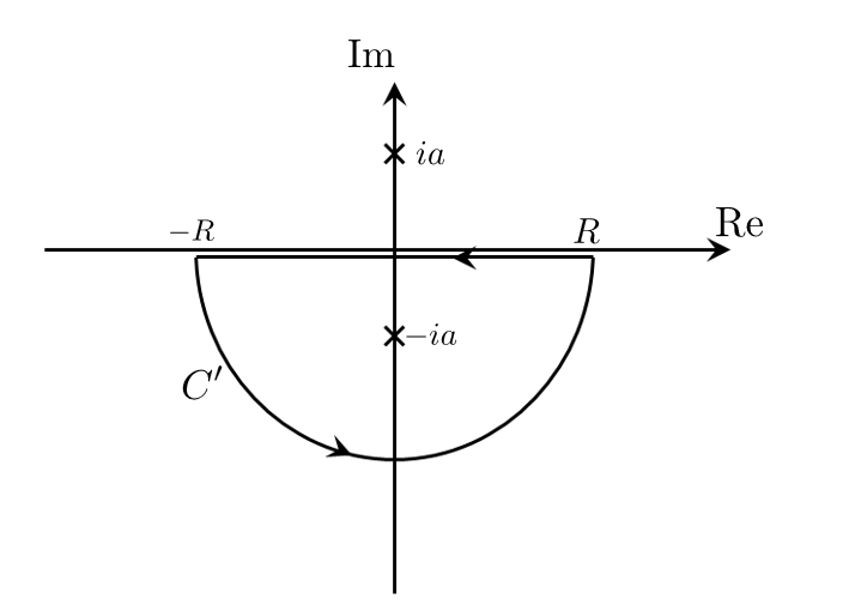
\includegraphics[width=.7\columnwidth]{Contour2.png}
  \caption{Contour $C^\prime$ for integration}
  \label{fig2}
\end{figure}




We repeat the same calculation using the different contour.
Since there are no singularities for $\displaystyle \frac{e^{izx}}{z-ia}$ inside the contour, we can apply Cauchy's Integral Theorem:
\begin{equation*}
  \frac{1}{2 \pi i} \oint_{C^\prime} \frac{e^{i z x}}{z-ia} \, dz = 0
\end{equation*}

Since $e^{izx}$ does not have singularity inside the contour, we can apply Cauchy's integral formula:
\begin{equation*}
  \frac{1}{2 \pi i} \oint_{C^\prime} \frac{e^{i z x}}{z+ia} \, dz = e^{a x}
\end{equation*}

Additionally, the above contour integrals can be written as
\begin{equation*}
  \frac{1}{2 \pi i} \oint_{C^\prime} \frac{e^{i z x}}{z-ia} \, dz 
  = \frac{1}{2 \pi i} \int_{R}^{-R} \frac{e^{i\xi x}}{\xi-ia} \, d\xi  + \frac{1}{2 \pi i} \int_{\pi}^{2 \pi} \frac{e^{i Re^{i \theta} x}}{Re^{i \theta}-ia} iRe^{i \theta} \, d \theta
  =0
\end{equation*}

\begin{equation*}
  \frac{1}{2 \pi i} \oint_{C^\prime} \frac{e^{i z x}}{z+ia} \, dz 
  = \frac{1}{2 \pi i} \int_{R}^{-R} \frac{e^{i\xi x}}{\xi+ia} \, d\xi  + \frac{1}{2 \pi i} \int_{\pi}^{2\pi} \frac{e^{i Re^{i \theta} x}}{Re^{i \theta}+ia} iRe^{i \theta} \, d \theta
  = e^{a x}
\end{equation*}

Here, we evaluate the following integral

\begin{equation*}
  \int_{\pi}^{2\pi} \frac{e^{i Re^{i \theta} x}}{Re^{i \theta} \pm ia} iRe^{i \theta} \, d \theta
\end{equation*}

\begin{align*}
  \left| \int_{\pi}^{2\pi} \frac{e^{i Re^{i \theta} x}}{Re^{i \theta} \pm ia} iRe^{i \theta} \, d \theta \right|
  & \leq \frac{R}{R-a}\int_{\pi}^{2\pi} e^{- R\sin \theta x} \, d \theta \quad \text{(The same calculation as $x>0$)}\\
  & =    \frac{R}{R-a}\int_{0}^{\pi} e^{R\sin \theta x} \, d \theta\\
  & =     \frac{R}{R-a}\int_{-\frac{\pi}{2}}^{\frac{\pi}{2}} e^{R\sin \left( \theta+\frac{\pi}{2}\right) x} \, d \theta\\
  & =     \frac{R}{R-a}\int_{-\frac{\pi}{2}}^{\frac{\pi}{2}} e^{R\cos \theta x} \, d \theta\\
  & =     \frac{2R}{R-a}\int_{0}^{\frac{\pi}{2}} e^{R\cos \theta x} \, d \theta \quad \text{($\cos \theta$ is an even function)}
\end{align*}

Since $\cos \theta \geq -\displaystyle \frac{2}{\pi} \theta + 1 \, \left( 0\leq \theta \leq \displaystyle \frac{\pi}{2} \right)$ and $x<0$,
\begin{align*}
  \left| \int_{\pi}^{2\pi} \frac{e^{i Re^{i \theta} x}}{Re^{i \theta} \pm ia} iRe^{i \theta} \, d \theta \right|
  & \leq  \frac{2R}{R-a}\int_{0}^{\frac{\pi}{2}} e^{R \left( -\frac{2}{\pi}\theta + 1 \right) x} \, d \theta \\
  & =     \frac{2Re^{Rx}}{R-a}\int_{0}^{\frac{\pi}{2}} e^{-R\frac{2}{\pi}\theta x} \, d \theta \\
  & =     \frac{2Re^{Rx}}{R-a}\left[ \frac{\pi}{2Rx}e^{-R\frac{2}{\pi}\theta x} \right]_{0}^{\frac{\pi}{2}}\\
  & =     \frac{\pi e^{Rx}}{\left(R-a\right) x}\left( e^{-Rx} - 1 \right)\\
  & =     \frac{\pi \left( 1 - e^{Rx} \right)}{\left(R-a\right) x} \rightarrow 0 \quad (R \rightarrow \infty)
\end{align*}

Therefore,
\begin{equation*}
  \lim_{R \rightarrow \infty}\left[ \frac{-1}{2 \pi i} \int_{-R}^{R} \frac{e^{i\xi x}}{\xi-ia} \, d\xi  + \frac{1}{2 \pi i} \int_{\pi}^{2\pi} \frac{e^{i Re^{i \theta} x}}{Re^{i \theta}-ia} iRe^{i \theta} \, d \theta\right]
  = \frac{-1}{2 \pi i} \int_{-\infty}^{\infty} \frac{e^{i\xi x}}{\xi-ia} \, d\xi = 0
\end{equation*}
\begin{equation*}
  \lim_{R \rightarrow \infty}\left[ \frac{-1}{2 \pi i} \int_{-R}^{R} \frac{e^{i\xi x}}{\xi+ia} \, d\xi  + \frac{1}{2 \pi i} \int_{\pi}^{2\pi} \frac{e^{i Re^{i \theta} x}}{Re^{i \theta}+ia} iRe^{i \theta} \, d \theta\right]
  = \frac{-1}{2 \pi i} \int_{-\infty}^{\infty} \frac{e^{i\xi x}}{\xi+ia} \, d\xi = e^{a x}
\end{equation*}
Hence, the Inverse Fourier Transform for $x<0$ is
\begin{align*}
  \mathcal{F}^{-1}  \left[ \hat{f} \right] \left( x \right) 
  &= \frac{1}{2 \pi i} \left[ \int_{-\infty}^{\infty} \frac{e^{i\xi x}}{\xi-ia} \, d\xi -  \int_{-\infty}^{\infty} \frac{e^{i\xi x}}{\xi+ia} \, d\xi \right] \\
  &= e^{a x}
\end{align*}

If $x=0$, 
The Inverse Fourier Transform is
\begin{align*}
  \mathcal{F}^{-1}  \left[ \hat{f} \right] \left( 0 \right) 
  &= \frac{1}{2 \pi} \int_{-\infty}^{\infty} \frac{2a}{a^2+\xi^2} \, d\xi \\
  &= \frac{a}{\pi} \int_{-\infty}^{\infty} \frac{1}{a^2+\xi^2} \, d\xi \\
  &= \frac{a}{\pi} \int_{-\frac{\pi}{2}}^{\frac{\pi}{2}} \frac{1}{a^2+a^2\tan^2 \phi} \frac{a}{\cos^2 \phi} \, d\phi \quad (\xi = a \tan \phi)\\
  &= \frac{1}{\pi} \int_{-\frac{\pi}{2}}^{\frac{\pi}{2}}  \, d\phi\\
  &= 1
\end{align*}

Therefore,
\[
  \mathcal{F}^{-1}  \left[ \hat{f} \right] \left( x \right)  =
  \begin{cases}
    e^{-a x} & \text{if } x>0 \\
    1 & \text{if } x=0\\
    e^{a x} & \text{if } x<0
  \end{cases}
\]

This is equivalent to
\begin{equation*}
  \mathcal{F}^{-1}  \left[ \hat{f} \right] \left( x \right)  = e^{-a|x|}
\end{equation*}
\end{document}